\documentclass[xcolor=dvipsnames]{beamer}
\usepackage{xmpmulti}
\usepackage{comp2402}
\usepackage{fancyvrb}


\title{Sorting and Sorting Lower Bounds}
\author{}
\date{}


\begin{document}

\begin{frame}
  \titlepage
  \begin{center}
    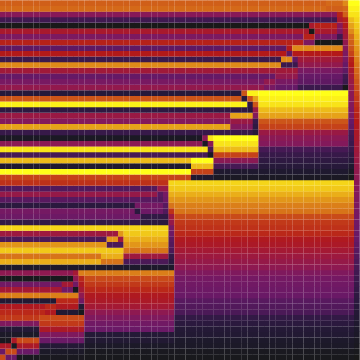
\includegraphics[height=1.2in]{images/merge-sort}
  \end{center}
\end{frame}

\begin{frame}
  \frametitle{The Merge Sort Algorithm}

  \begin{tabular}{p{2.5in}p{1in}}
  \begin{itemize}
    \item<+->Used in J. W. Bryce's Sorting maching in 1938 (U.S. Patent 2189024)
    \item<+->``Invented'' by John von Neumann in 1945
    \item<+->To sort $#a[0]#,\ldots,#a[n-1]#$:
    \begin{enumerate}
      \item<+-> sort $#a[0]#,\ldots,#a[n/2]#$
      \item<+-> sort $#a[n/2+1]#,\ldots,#a[n-1]#$
      \item<+-> merge the two sorted sequences
    \end{enumerate}
  \end{itemize}
  &
  \begin{center}
    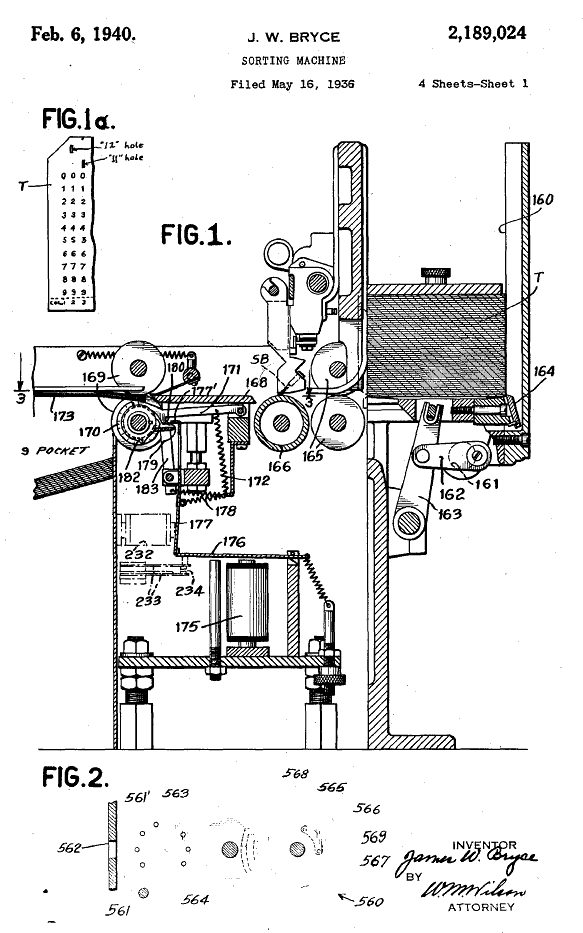
\includegraphics[height=1.5in]{images/sorting}
  \end{center}
  \end{tabular}
\end{frame}


\begin{frame}

  \frametitle{Mergesort}
  \begin{itemize}
    \item<+->To sort $#a[0]#,\ldots,#a[n-1]#$:
    \begin{enumerate}
      \item<+-> sort $#a0=a[0]#,\ldots,#a[n/2]#$  (recursively)
      \item<+-> sort $#a1=a[n/2+1]#,\ldots,#a[n-1]#$ (recursively)
      \item<+-> merge the two sorted sequences
    \end{enumerate}
    \item<+-> $\langle 9, 3, 5, 2, 1, 8, 7, 0, 6, 4 \rangle$
    \item<+->
     \only<1>{$\langle 9, 3, 5, 2, 1\rangle \langle 8, 7, 0, 6, 4 \rangle$}%
     \only<2>{$\langle 1, 2, 3, 5, 9\rangle \langle 8, 7, 0, 6, 4 \rangle$}
     \only<+->{$\langle 1, 2, 3, 5, 9\rangle \langle 0, 4, 6, 7, 8 \rangle$}
    \item<+->$\langle 0, 1, 2, 3, 4, 5, 6, 7, 8, 9\rangle$
  \end{itemize}
\end{frame}

\begin{frame}[fragile]
  \frametitle{Mergesort}
  \javaimport{ods/Algorithms.mergeSort(a,c)}
\end{frame}

\begin{frame}[fragile]
  \frametitle{Merging two sorted arrays}

  \begin{itemize}
    \item<+-> To merge two sorted arrays (or lists) #a# and #b# we scan
    them sequentially
    \javaimport{ods/Algorithms.merge(a0,a1,a,c)}
    \item<+-> Takes $O(#n#)$ time
  \end{itemize}
\end{frame}

\begin{frame}
  \frametitle{Analysis of Mergesort}

  \begin{itemize}
    \item<+->Mergesort $#a[0]#,\ldots,#a[n-1]#$:
    \begin{enumerate}
      \item<+-> sort $#a[0]#,\ldots,#a[n/2]#$  (recursively)
      \item<+-> sort $#a[n/2+1]#,\ldots,#a[n-1]#$ (recursively)
      \item<+-> merge the two sorted sequences
   \end{enumerate}
   \item<+-> Let $T(#n#)$ be the time to run merge sort on an array of length $n$
   \item<+-> Step 1 Takes $T(#n#/2)$ time
   \item<+-> Step 2 Takes $T(#n#/2)$ time
   \item<+-> Step 3 Takes $O(#n#)$ time
   \item<+-> $T(#n#) = O(#n#) + 2T(#n#/2)$\footnote{Cheating a bit here, assuming $n$ is a power of 2.}
  \end{itemize}
\end{frame}

\begin{frame}
  \frametitle{The Mergesort recurrence}

  \begin{itemize}
    \item<+-> $T(#n#) = O(#n#) + 2T(#n#/2)$
    \item<+->\only<2>{$T(#n#) = O(#n#) + 2O(#n#/2) + 4T(#n#/4)$}%
             \only<+->{$T(#n#) = O(#n#) + O(#n#) + 4T(#n#/4)$}%
    \item<+->\only<4>{$T(#n#) = O(#n#) + O(#n#) + 4O(#n#/4) + 8T(#n#/8)$}%
             \only<+->{$T(#n#) = O(#n#) + O(#n#) + O(#n#) + 8T(#n#/8)$}%
    \item<+->\only<6>{$T(#n#) = O(#n#) + O(#n#) + O(#n#) + \cdots + #n#O(1)$}%
             \only<+->{$T(#n#) = O(#n#) + O(#n#) + O(#n#) + \cdots + O(#n#)$}
    \item<+->$T(#n#) = O(#n#\log #n#)$
    \item<+->\textbf{Theorem:} The Mergesort algorithm can sort an array of $#n#$ items in $O(#n#\log #n#)$ time
  \end{itemize}
\end{frame}

\begin{frame}
  \frametitle{Reminder: Mergesort}
  \begin{center}
    \includegraphics[height=2in]{figs/mergesort}
  \end{center}
  \begin{itemize}
  \item<+->Mergesort sorts an array of #n# elements in $O(#n#\log #n#)$ worst-case time using at most $#n#\log #n#$ comparisons
  \end{itemize}
\end{frame}

\begin{frame}
  \frametitle{Reminder: Quicksort}
  \begin{center}
    \includegraphics{figs/quicksort}
  \end{center}
  \begin{itemize}
    \item<+->Quicksort sorts an array of #n# elements in $O(#n#\log #n#)$ expected     time using at most $1.38#n#\log #n#$ expected comparisons
  \end{itemize}
\end{frame}

\begin{frame}
  \frametitle{Reminder: Heapsort}
  \begin{center}
    \includegraphics{figs/heapsort}
  \end{center}
  \begin{itemize}
  \item<+->Heapsort sorts an array of #n# elements in $O(#n#\log #n#)$ worst-case time using at most $2#n#\log #n#$ comparisons
  \end{itemize}
\end{frame}


\begin{frame}
  \frametitle{Comparison-based sorting algorithms}

  \begin{itemize}
    \item<+-> So far, we have seen 3 sorting algorithms:
    \begin{itemize}
      \item<+-> Quicksort: $O(#n#\log #n#)$ expected time
      \item<+-> Heapsort: $O(#n#\log #n#)$ time
      \item<+-> Mergesort: $O(#n#\log #n#)$ time
    \end{itemize}
    \item<+-> Is there a faster (maybe $O(#n#)$ time) sorting algorithm?
    \begin{itemize}
      \item<+-> Answer: No and yes
    \end{itemize}
  \end{itemize}

\end{frame}

\begin{frame}
  \frametitle{Comparison-based sorting algorithms}

  \begin{itemize}
    \item<+-> Quicksort, Heapsort, and Mergesort are comparison-based
    \begin{itemize}
      \item<+-> All branching in the algorithm is based on the results
        of comparisons of the form $#a[i] < b[i]#$
      \item<+-> These algorithms can be used to sort any array of
        #Comparable# items
      \item<+-> But this comes at a price
      \begin{itemize}
        \item<+-> Every comparison-based sorting algorithm takes $\Omega(#n#\log #n#)$ time for some input
      \end{itemize}
    \end{itemize}
  \end{itemize}
\end{frame}


\begin{frame}
  \frametitle{Comparison trees}

  \begin{itemize}
    \item<+-> A \emph{comparison tree} is a full binary tree:
    \begin{itemize}
      \item<+-> each internal node #u# is labelled with a pair #u.i# and #u.j# 
      \item<+-> each leaf is labelled with a permutation of $\{0,\ldots,n-1\}$ 
    \end{itemize}
    \item<+-> For an array #a# we can \emph{run} the comparison tree   
    \begin{itemize}
      \item<+-> #u# is the root
      \item<+-> while #u# is not a leaf
      \begin{itemize}
        \item<+-> if $a[u.i] < a[u.j]$ then #u = u.left# else #u = u.right#
      \end{itemize}
    \end{itemize}
    \item<+-> The comparison tree \emph{sorts} if, for every input array #a#, the permutation at the leaf for #a# correctly sorts #a#
  \end{itemize}
\end{frame}

\begin{frame}
  \frametitle{Comparison tree example}
  \begin{center}
   \includegraphics[width=\textwidth]{figs/comparison-tree}
  \end{center}
\end{frame}


\begin{frame}
  \frametitle{Comparison tree lower bound}
  
  \begin{itemize}
  \item<+->\textbf{Lemma:} Every comparison tree that sorts any input of length $#n#$ has at least $#n#!$ leaves
  \item<+->\textbf{Theorem:} Every comparison tree that sorts any input of length $#n#$ has height at least $(#n#/2)\log_2 (#n#/2)$ 
  \begin{itemize}
    \item<+-> The height of a tree with $m$ leaves is at least $\log_2 m$
    \item<+-> The height of a tree with $#n#!$ leaves is at least $\log_2 #n#!$
    \item<+->[]
      
        \begin{eqnarray*} 
          \log_2 #n#!& =& \log_2(#n#) + \log_2(#n#-1) + \cdots+\log_2(1) \\
                   &\ge&\log_2(#n#) + \cdots+\log_2(#n#/2) \\
                   &\ge&\log_2(#n#/2) +\cdots+\log_2(#n#/2) \\
                   &=&(#n#/2)\log_2(#n#/2)
        \end{eqnarray*}
   \end{itemize}
  \item<+> Lower bound can be improved to $#n#\log #n# - O(#n#)$
  \end{itemize}
\end{frame}


\begin{frame}
  \frametitle{Comparison tree lower bound}

  \begin{center}
   \includegraphics[width=\textwidth]{figs/comparison-tree-b}
  \end{center}
  \begin{itemize}
    \item<+-> Does not sort correctly because
    \begin{itemize}
      \item<+-> $3!=3\cdot 2\cdot 1=6$
      \item<+-> this tree has only $4<6$ leaves
    \end{itemize}
  \end{itemize}
\end{frame}
 
\begin{frame}
  \frametitle{Comparison-based sorting and comparison trees}

  \begin{itemize}
    \item<+->Every deterministic comparison-based sorting algorithm $\mathcal{A}$ that can sort every array of $n$ elements defines a comparison tree $T_\mathcal{A}$ that sorts
    \item<+->The height of $T_\mathcal{A}$ is equal to the (worst-case) number of comparisons that $\mathcal{A}$ performs
    \item<+->\textbf{Theorem:} For every deterministic comparison-based sorting algorithm $\mathcal{A}$, there exists an input such that $\mathcal{A}$ requires $\Omega(#n#\log #n#)$ comparisons
    \item<+->\textbf{Theorem:} For every comparison-based sorting algorithm $\mathcal{A}$, the expectedd number of comparisons performed by $\mathcal{A}$ while sorting a random permutation is $\Omega(#n#\log#n#)$
  \end{itemize}
\end{frame}


\begin{frame}
  \frametitle{Summary}

  \begin{itemize}
    \item<+-> Mergesort: runs in $O(#n#\log #n#)$ time
    \item<+-> Any comparison-based sorting algorithm requires $\Omega(#n#\log #n#)$ time
    \item<+-> Mergesort, Quicksort, and Heapsort are optimal comparison-based sorting algorithms
    \item<+-> In-class problem:
    \begin{itemize}
      \item<+-> Design an algorithm that takes an array #a# of #n# integers in the range $\{0,\ldots,#k#-1\}$ and sorts them in $O(#n#+#k#)$ time
    \end{itemize}
  \end{itemize}
\end{frame}

\begin{frame}[fragile]
  \frametitle{Counting sort}

  \javaimport{ods/Algorithms.countingSort(a,k)}
\end{frame}

\begin{frame}[fragile]
  \frametitle{Counting sort}

  \begin{center}
    \includegraphics[height=2in]{figs/countingsort}
  \end{center}
  \begin{itemize}
   \item<+->\textbf{Theorem:} The counting sort algorithm can sort an array #a# of #n# integers in the range $\{0,\ldots,#k#-1\}$ in $O(#n#+#k#)$ time
  \end{itemize}
\end{frame}

\begin{frame}[fragile]
  \frametitle{Radix sort}
  \begin{itemize}
    \item<+-> Radix-sort uses the counting sort algorithm to sort integers one ``digit'' at a time
    \begin{itemize}
      \item<+-> integers have #w# bits
      \item<+-> ``digit'' has #d# bits
      \item<+-> uses $#w#/#d#$ passes of counting-sort
    \end{itemize}
    \item<+-> Starts by sorting least-significant digits first
    \begin{itemize}
      \item<+-> works up to most significant digits
    \end{itemize}
    \item<+-> Correctness depends on fact that counting sort is \emph{stable}
    \begin{itemize}
      \item<+-> if #a[i]=a[j]# and #i<j# then #a[i]# appears before #a[j]#
        in the output
    \end{itemize}
  \end{itemize}
\end{frame}

\begin{frame}[fragile]
  \frametitle{Counting sort}

  \begin{center}
    \includegraphics[width=\textwidth]{figs/radixsort}
  \end{center}
  \begin{itemize}
   \item<+->\textbf{Theorem:} The radix-sort algorithm can sort an array #a# of #n# #w#-bit integers in $O(#n#+2^{#d#})$ time
   \item<+->\textbf{Theorem:} The radix-sort algorithm can sort an array #a# of #n# integers in the range $\{0,\ldots,#n#^{c}-1\}$ in $O(c#n#)$ time.
  \end{itemize}
\end{frame}

\begin{frame}[fragile]
  \frametitle{Summary}
  \begin{itemize}
    \item<+-> Quicksort, Heapsort, and Mergesort can each sort an array of length #n# in $O(#n#\log #n#)$ time
    \begin{itemize}
      \item<+-> These work for any #Comparable# data type
      \item<+-> Quicksort and Heapsort are \emph{in-place} but do more comparisons
      \item<+-> Mergesort requires an auxiliary array
    \end{itemize}
    \item<+-> Radix-sort can sort an array #a# of #n# integers in the range $\{0,\ldots,#n#^{c}-1\}$ in $O(c#n#)$ time (and does no comparisons).
  \end{itemize}
\end{frame}

\end{document}

